% This is LLNCS.DEM the demonstration file of
% the LaTeX macro package from Springer-Verlag
% for Lecture Notes in Computer Science, version 1.1
\documentclass{llncs}
%\usepackage[numbers, sort&compress, square, comma]{natbib}
% \usepackage[lsnumbers, sort&compress, sEquare, comma]{natbib}    
% \usepackage{multirow}                             % not available on your system
\usepackage[table]{xcolor}
% \usepackage{amssymb}
\usepackage{amsmath}
\usepackage{graphicx}        % standard LaTeX graphics tool                            % when including figure files
\usepackage{multicol}        % used for the two-column index
\usepackage{multirow}
\usepackage{lscape}
\usepackage{float}
\usepackage{url}
\usepackage{caption,subfig}
\usepackage{graphicx}
\usepackage{amsmath}
\usepackage{amssymb}
\usepackage{color}
\usepackage{algorithm}
\usepackage{algorithmic}
\usepackage{tikz,graphicx}
\usepackage{url}
%\usepackage{etoolbox}
%\AtBeginEnvironment{algorithmic}{\small}
%



\graphicspath{{pictures/}} % Specifies the directory where pictures are stored

\def\dae{{\em Divide-and-Evolve}}
\def\DAE{{\sc DaE}}
\def\DAEX{{\sc DaE$_{\text{X}}$}}
%\def\DAEYAHSP{{\sc DaE$_{\text{YAHSP}}$}}
\newcommand{\DAEYAHSP}{{\sc DaE$_{\text{YAHSP}}$}}
\def\PARADISEO{{\sc ParadisEO-MOEO}}
\def\YAHSP{{\sc YAHSP}}
\def\modae{{\em Multi-Objective Divide-and-Evolve}}
\def\MODAE{{\sc MO-DaE}}
\def\ZENO{{\sc ZenoTravel}}
\def\MULTIZENO{{\sc MultiZenoTravel}}
\def\ZENOSOLVER{{\sc ZenoSolver}}
\def\PARAMILS{{\sc ParamILS}}

\newcommand{\mycomment}[1]{{\bf \textcolor{red}{#1}}}
\newcommand{\alexcomment}[1]{{\bf \textcolor{blue}{#1}}}


\begin{document}
%% Please leave SVN version number $Revision: 1002 $
% Remember to enter the SVN command 
%      svn propset svn:keywords "Revision" thisFile.tex
\setlength{\parskip}{0pt}
\setlength{\parsep}{0pt}
\setlength{\headsep}{0pt}
\setlength{\topskip}{0pt}
\setlength{\topmargin}{0pt}
\setlength{\topsep}{0pt}
\setlength{\partopsep}{0pt}

\title{Pareto Fronts for \MULTIZENO\ Benchmarks} % -- $Revision: 1002 $}

\author{A. Quemy \inst{1} \and M. Schoenauer\inst{1}\and
V. Vidal\inst{2}  \and J. Dr\'eo\inst{3} \and 
P. Sav\'eant\inst{3}}
% \author{Mostepha~R. Khouadjia \inst{1} \and Marc Schoenauer\inst{1}\and
% Vincent Vidal\inst{2}  \and Johann Dr\'eo\inst{3} \and Pierre Savéant\inst{3}}
%
\authorrunning{Alexandre Quemy et \textit{al.}} % abbreviated author list (for running head)
%
%%%% list of authors for the TOC (use if author list has to be modified)
\tocauthor{Alexandre Quemy, Marc Schoenauer, Vincent Vidal, Johann Dr\'eo, and Pierre Sav\'eant}
%
\institute{TAO Project, INRIA Saclay \&  LRI Paris-Sud University, Orsay, France\\%Universit\'{e} Paris-Sud
\email{\{alexandre.quemy, marc.schoenaue\}@inria.fr},\\ %WWW home page:
%\texttt{http://users/\homedir iekeland/web/welcome.html}
\and
ONERA-DCSD, Toulouse, France\\
\email{Vincent.Vidal@onera.fr}\\
 \and
 THALES Research \& Technology, Palaiseau, France\\
 \email{\{johann.dreo, pierre.saveant@thalesgroup.com\}}\\
}

\maketitle

\begin{abstract}
Contrary to single objective planning, multi-objective planning suffers from a lack of benchmarks with a known Pareto Front. As a result, testing and comparing algorithms is almost impossible. A method to generate various size tunable benchmarks for multi-objective planning with a known Pareto Front is proposed in order to provide a wide range of Pareto front shapes and different magnitudes of difficulty. The performances of the implementation are shown and some large instances with singular Pareto front shapes are proposed. A first attempt to solve some of them using multi-objective \DAEYAHSP\ solver is provided.
\end{abstract}
%
\section{Introduction}
\label{sec:intro}

Many benchmark suites exist for continuous multi-objective optimization (the famous ZDT, IHR, etc, proposed two decades ago), for which the exact Pareto front can be analytically computed, and with know difficulties (e.g. dimensionality, shape of the Pareto fronts, existence of local Pareto-optima, \ldots). For combinatorial optimization, the situation is not yet so clear, and whereas there exist known benchmark problems of all sizes, their Pareto fronts are generally not precisely known except the simplest ones (see e.g., MOCOLIB\footnote{\url{http://www.mcdmsociety.org/MCDMlib.html}}, offering several instances of several well-known combinatorial benchmark problems).

The context of the proposed benchmark suite is that of AI planning: a planning domain is defined by a set of predicates, that define the state of the system, a set of possible actions that can be triggered in states where their pre-conditions are satisfied, resulting in a new state. A planning problem instance is defined on a given planning domain by a list of objects, used to instantiate the predicates to define the state, an initial and a target state. The goal is to some up with a {\em feasible plan}, i.e., a set of actions that, when applied in turn to the initial state, lead the system to the goal state.

A simple planning problem in the domain of logistics, inspired by the well-known {\ZENO} problem of IPC series (see Figure \ref{fig.instance}) involves cities, passengers, and planes. Planes can fly from one city to another when a link exist, taking a given duration to do so (number on the link). Planes fly either empty, or carrying a unique passenger. An instance is defined by the number of cities and the links between them, a number of passengers and a number of planes. The goal of the (single-objective) planning problem is to carry all passengers from city I to city G in the minimum {\em makespan} (total duration of all flights). Because all planes can of course fly in parallel, this benchmark pertains to temporal planning. Previous work \cite{khouadjia:hal-00750560} proposed a multi-objective version of these benchmarks called \MULTIZENO, by adding a {\em cost} for landing in some cities: the second objective is to minimize the {\em total cost} of the plan. This work demonstrated the possibility for such 
problems to provide Pareto Front of various shapes and difficulties, but only provided the exact Pareto front for small instances.

This paper analyzes the \MULTIZENO\ benchmarks, providing an algorithm to compute the true Pareto Front even for very large instances. Beyond providing a generic way to generate Pareto Fronts of diverse complexities for AI Planning, the proposed \MULTIZENO\ benchmarks will allow testing different generic decomposition methods (weighted sum aggregation, Tchebycheff decomposition, Boundary Intersection approach -- see e.g., \cite{Zhang-MOEAD-TEC07}) on large, concave, non-uniform, \ldots benchmarks of Combinatorial Multi-objective Problems of for which the Pareto Front is exactly known. 

The paper is organized as follows: Section \ref{sec:multizeno} formally presents the  \MULTIZENO\ benchmark, proving some properties of their Pareto optimal plans. Building on these properties, Section \ref{sec:zenosolver} proposes the \ZENOSOLVER\ algorithm to actually derive the true Pareto front for these instances. Sample experimental results demonstrate the diversity of Pareto fronts that can be obtained, and gives performance measurements of its complexity on large instances. The end of the paper presents experiments on some of the large \MULTIZENO\ instances obtained by Divide-and-Evolve, the only Pareto-based evolutionary AI planner to-date \cite{IJCAI2013}, which is rapidly recalled in Section \ref{sec:exp}, before some comparison with its single-objective version using the weighted sum aggregation on problems with non-convex fronts are given and discussed in Section \ref{sec:exp}.

\section{\MULTIZENO\ problem}
\label{sec:multizeno}
\subsection{Instances}



Let us introduce some notations related to the planning problems introduced in Section \ref{sec:intro}: a \MULTIZENO\ instance (Figure \ref{fig.instance}) is defined by: $n$ 'central' cities, with costs $c_1, \ldots, c_n$\footnote{by simplicity, $c_i$ will denote both the city and the cost of landing in that city.}, plus the initial and goal cities $c_I$ and $c_G$; $t$ persons and $p$ planes, initially in $c_I$. Each central city provides a flight to the initial and final cities, with same flight durations $d_1, \ldots, d_n$. In addition, central cities form a clique, with durations $(d_{ij})_{i,j}, \forall (i,j) \in [1,n]^2$. The goal is to carry all persons to $c_G$, minimizing the makespan and the total cost of the plan.
Let us analyze some properties of the Pareto fronts of such problems, that will allow us to design an efficient algorithm to actually compute them in a reasonable time.
\begin{figure}
\centering
 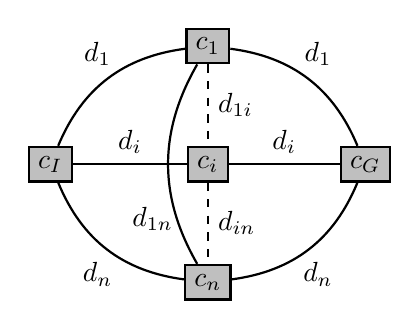
\begin{tikzpicture}[thick,scale=1]
     % Villes
  \node[draw, fill=black!25] (0) at (-2,0) {$c_I$};
  \node[draw, fill=black!25] (1) at (0,1.5) {$c_1$};
  \node[draw, fill=black!25] (2) at (0,0) {$c_i$};
  \node[draw, fill=black!25] (3) at (0,-1.5) {$c_n$};
  \node[draw, fill=black!25] (4) at (2,0) {$c_G$};
 
     % Liaison inter villes
  \draw[thick] (0) to[bend left] (1);
  \draw[thick] (0)--(2) node[midway, above]{$d_i$};
  \draw[thick, bend left] (0) to[bend right] (3);
  
  \draw[thick] (1) to[bend left] (4);
  \draw[thick] (2)--(4) node[midway, above]{$d_i$};
  \draw[thick] (3) to[bend right] (4);
  
  \draw[dashed] (1)--(2) node[midway, right]{$d_{1i}$};
  \draw[dashed] (2)--(3) node[midway, right]{$d_{in}$};
  \draw[thick] (1) to[bend right] (3);
     
     % Distance particulière
  \node[] (A) at (-1.4,1.4) {$d_1$};
  \node[] (A) at (1.4,1.4) {$d_1$};
  \node[] (A) at (-1.4,-1.4) {$d_n$};
  \node[] (A) at (1.4,-1.4) {$d_n$};
  \node[] (A) at (-0.7,-0.7) {$d_{1n}$};
  
\end{tikzpicture}
%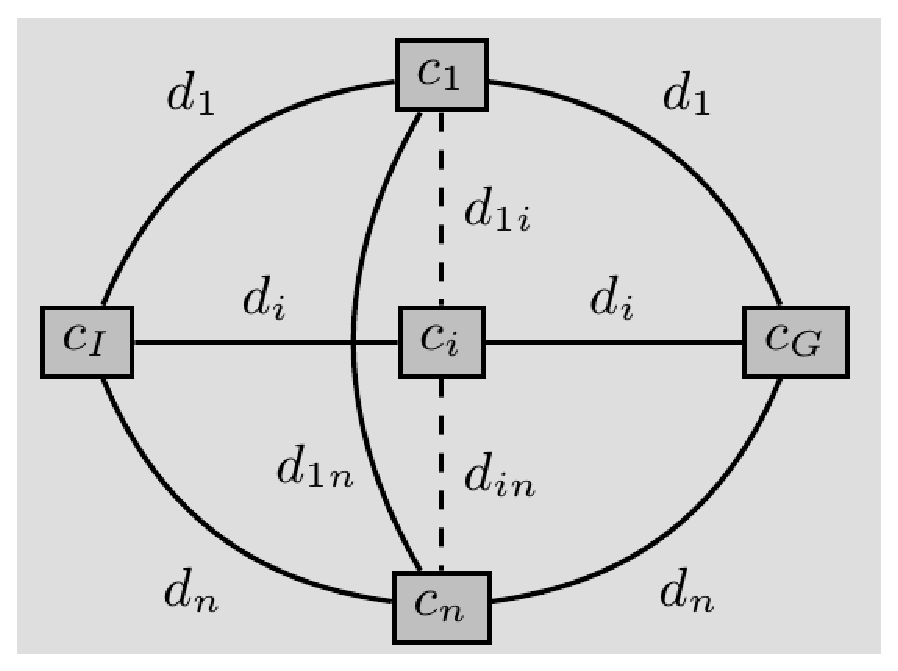
\includegraphics[width=0.5\textwidth]{abstractZeno.eps}
\caption{\label{fig.instance}A schematic view of a general \MULTIZENO\ problem. }
\end{figure}
%Without loss of generality, we can assume that the pairs $(d_i, c_i)$ are pairwise distinct (otherwise, the 2 cities can be ``merged'' and the resulting $n-1$ cities problem is equivalent to the original $n$ cities problem).

\subsection{Pareto Optimal Plans}

\noindent
{\bf Hypothesis}: Assume that, for all pair of cities $(i,j)$, $d_i + d_j < d_{ij}$\footnote{Even though this might look unrealistic in real-world logistic domain. However, we hypothesize that the result still holds with the weaker condition that for any cities $c_i, c_j, c_k$ ($c_0=I$ and $c_{n+1}=G$), $d_{ik} \leq d_{ij} + d_{jk}$ (triangular inequality).}. Then the following holds.

\noindent
{\bf Proposition}: Pareto-optimal plans are plans where exactly $2t-p$ central cities are reached by a flight.

\noindent
{\bf Proof}:
Consider a plan where a person flies from $c_i$ to $c_j$. Using the same plane, the same person could fly instead from $c_i$ to $c_G$, and the plane would return empty to $c_j$. The plan could continue unchanged from thereon: because of the hypothesis on makespans, the needed resource would be in $c_j$ on time. Moreover, the total cost is unchanged, and the total makespan is lower or equal to the original one: the new plan thus Pareto-dominates the original one.

Iterating the same reasoning for each person, and each empty plane, we conclude that there are no flights between central cities in Pareto-optimal plans. Thus bringing the $t$ persons from $c_I$ to $c_G$ will amount to carry each person through one central city: $t$ flights will be needed from $c_I$ to one $c_i$, then $t$ flights from $c_i$ to $c_G$. Of course, $t-p$ flights back empty will be needed for some planes, possibly through some different central cities-- hence the result. \hfill $\square$\\

\noindent
{\bf Counting and Pruning Possibly Pareto-optimal Plans.}
A Possibly Pareto-optimal Plan (PPP) is thus defined by 2 tuples, namely $e \in [1,n]^t$ for cities involved in eastbound flights, and $w \in [1,n]^{t-p}$ for westbound flights, and the optimal  schedule for the $p$ planes along the corresponding $4t-2p$ arcs. However, such definition contains redundancies, that are removed by ordering the indices:\\

\noindent
{\bf Definition}: An {\it admissible PPP} is a pair of $E \times W$, where $E = \{e \in [1,n]^t ; \forall i \in [1,t-1], d_{e_i} \geq d_{e_{i+1}}\}$ and $W = \{w \in [1,n]^{t-p} ; \forall i \in [1,t-p-1],  d_{w_i} \geq d_{w_{i+1}}\}$.\\

\noindent
{\bf Number of admissible PPPs}: Let $K^{m}_{k}$ be the set of $k$-multicombinations (or multi-subset of size $k$) with elements in a set of of size $m$. The cardinality of $K^{m}_{k}$ is $\Gamma^{m}_{k} = {m+k-1 \choose k}$. As $E$ is in bijection with $K^{n}_{t}$, and $K^{n}_{t-p}$ with $W$, the number of PPP is $\Gamma^{n}_{t} \Gamma^{n}_{t-p}$, i.e., ${n+t-1 \choose t}{n+(t-p)-1 \choose t-p}$.\\

\noindent
{\bf Cost of a PPP}: Given the PPP $(e,w) \in E \times W$, the cost of {\bf any} plan using only the cities in $e$ and $w$ is $\text{Cost}(C) = \underset{{e_i \in e}}{\sum} c_{e_i} + \underset{{w_i \in w}}{\sum} c_{w_i}$.\\

\noindent
{\bf Makespan of a PPP}: The makespan of a PPP is thus that of the shortest schedule that uses exactly the $4t-2p$ arcs in a feasible way. Trivial upper and lower bounds for the shortest makespan of PPP $C$ are respectively $M_S(C)$, the makespan of the sequential plan (i.e., that of the plan for a single plane that would carry all persons one by one), and $M_L(C)$, the makespan of the perfect plan where none of the $p$ planes would ever stay idle. These bounds will be useful to prune PPP.

$$M_S(C) = 2 (\underset{{e_i \in e}}{\sum} d_{e_i} + \underset{{w_i \in w}}{\sum} d_{w_i}) ~~~~~~~~~~~~~~~~ M_L(C) = \frac{M_S(C)}{p}$$

\noindent
{\bf Greedy (Pareto) domination}: Given two PPP $C$ and $C'$, $C$ {\it greedily dominates} $C'$ if $M_S(C) \leq M_L(C')$ and $\mbox{Cost}(C) \leq \mbox{Cost}(C')$.

\subsection{Computing the Shortest Makespan} \label{computingMakespan}
%\subsubsection{Flight patterns}

% \begin{figure}
% \centering
% \begin{tikzpicture}[thick,scale=0.4]
%     % Villes
%  \node[draw, fill=black!25] (0) at (-3.5,0) {\large $c_0$};
%  \node[draw, fill=black!25] (2) at (0,0) {\large $c_i$};
%  \node[draw, fill=black!25] (4) at (3.5,0) {\large $c_G$};
% 
%     % Liaison inter villes
%  \draw[thick] (0)--(2) node[midway, above]{$d_{i}$};
%  \draw[thick] (2)--(4) node[midway, above ]{$d_{i}$};
% 
%  \draw[thick,->,>=stealth, red] (0.20) -- (2.160);
%  \draw[thick,->,>=stealth, red] (2.20) -- (4.160);
% \end{tikzpicture}
% %\caption{\label{M1} Pattern 1}
% \begin{tikzpicture}[thick,scale=0.4]
%     % Villes
%  \node[draw, fill=black!25] (0) at (-3.5,0) {\large $c_0$};
%  \node[draw, fill=black!25] (2) at (0,0) {\large $c_i$};
%  \node[draw, fill=black!25] (4) at (3.5,0) {\large $c_G$};
% 
%     % Liaison inter villes
%  \draw[thick] (0)--(2) node[midway, above]{$d_{i}$};
%  \draw[thick] (2)--(4) node[midway, above]{$d_{i}$};
% 
%  \draw[thick,<-,>=stealth, red] (0.20) -- (2.160);
%  \draw[thick,<-,>=stealth, red] (2.20) -- (4.160);
% \end{tikzpicture}
% %\caption{\label{M2} Pattern 2}
% \begin{tikzpicture}[thick,scale=0.4]
%     % Villes
%  \node[draw, fill=black!25] (0) at (-3.5,0) {\large $c_0$};
%  \node[draw, fill=black!25] (2) at (0,0) {\large $c_i$};
%  \node[draw, fill=black!25] (4) at (3.5,0) {\large $c_G$};
% 
%     % Liaison inter villes
%  \draw[thick] (0)--(2) node[midway, above]{$d_{i}$};
%  \draw[thick] (2)--(4) node[midway, above]{$d_{i}$};
% 
%  \draw[thick,->,>=stealth, red] (0.20) to[left] (2.160);
%  \draw[thick,<-,>=stealth, red] (0.-20) to[right] (2.200);
% 
%   \draw[thick,->,>=stealth, blue] (2.380) to[left] (4.160);
%  \draw[thick,<-,>=stealth, blue] (2.340) to[right] (4.200);
% \end{tikzpicture}
% \caption{\label{M3} Respectively Pattern 1,2 and 3.}
% \end{figure}


% \begin{figure}
% \centering
% 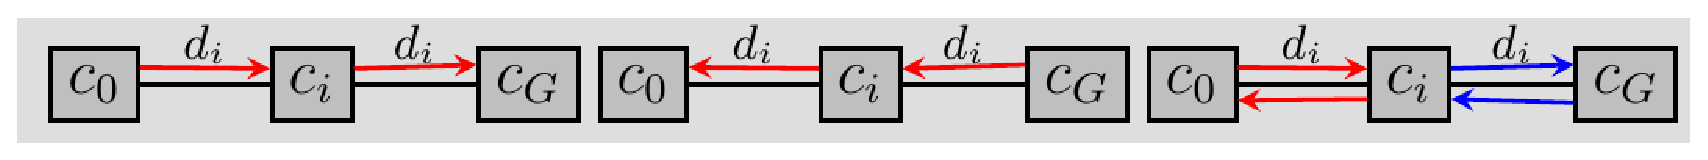
\includegraphics[width=0.8\textwidth]{patternsZeno.eps}
% \caption{\label{M3} Respectively Pattern 1,2 and 3.}
% \end{figure}
%,->,>=stealth
Clearly, all possible plane moves during the execution of a PPP can be categorized into the following 3 patterns: \\
%  represented on Fig. \ref{M3}. 
{\bf P1}: plane leaves $I$ (with passenger), flies eastward to city $c_i$, and goes on to $G$;\\
{\bf P2}: plane leaves $G$ (empty), flies westward to city $c_i$, and goes on to $G$;\\
{\bf P3}: two planes are involved here; first plane leaves $I$ (with passenger), flies to city $c_i$, and goes back empty to $I$; second plane leaves $G$ empty, flies to $c_i$, and flies back with the passenger to $G$. Note that there can be some delay between the drop-off of the person at the central city, and the arrival of the second plane.

Let $\alpha_E$,  $\alpha_W$, and $\beta$ be the numbers of patterns P1, P2, and P3 respectively. Clearly, $\beta$ entirely determines $\alpha_E$ and  $\alpha_W$, as $\alpha_W = t-p-\beta$ and $\alpha_E = t - \beta$.

Notice that, given $\beta$, there are multiple choices for the cities involved in the different P3. Each choice (list of cities) will be called a $\beta_{set}$, and the set of all possible $\beta_{set}$ is called the $\beta$-PowerSet. 


%\subsubsection{The method}
The optimal makespan of a given admissible PPP $C$ for a given $\beta$ is the lowest makespan obtained among all $\beta_{set} \in \beta$-PowerSet. For each $\beta_{set}$, the idea is to first solve the subproblem obtained by removing all P3s, and then to account for them in a second step. 
We shall prove that the obtained makespan is optimal.\\
%\subsubsection{Subproblem} 

\noindent
{\bf First Step}: The greedy Algorithm \ref{greedyAlgo} returns the optimal makespan for a PPP without any P3 (i.e., with $\beta = 0$), allocating the longest durations first.
Consider now a PPP $C = (e,w)$ and $\beta_{set}$, let $e' = e \backslash \beta_{set}$  and $w' = w \backslash \beta_{set}$ (obtained by removing the elements of $\beta_{set}$ from $e$ and $w$). The new PPP $C'=(e',w')$ has by definition no P3, and it can be applied Algorithm \ref{subproblem}. As we need them for the second step, the algorithm return durations $(D_i)_i$ for all planes. The optimal makespan of $C'$ is obviously $\max_i(D_i)$.


\begin{algorithm}[tb]
\caption{\label{subproblem} Computing the optimal makespan when $\beta = 0$}
\begin{algorithmic}\label{greedyAlgo}
%\REQUIRE $n \geq 0 \vee x \neq 0$
%\ENSURE $y = x^n$
\STATE $maxE \leftarrow 1$ ; $maxW \leftarrow t+1$ \hfill \COMMENT{Start with longest durations both sides}
\STATE $D_i \leftarrow 0 \; \forall i=1,\ldots,p$ \hfill\COMMENT{'Private' makespan for plane i}
\STATE $S_i \leftarrow EAST \; \forall i=1,\ldots,p$ \hfill
\COMMENT {Direction for next flight of plane i}

\WHILE{$maxW \leq 2t-p$}
\STATE $k \leftarrow {\mbox{ArgMin}_i}(D_i)$ \hfill \COMMENT {Schedule next in line (in $c_I$ or $c_G$)}
\IF{$S_k = EAST$}
\STATE $D_k \leftarrow D_k + 2d_{e_{maxE}}$\hfill
\STATE $S_k \leftarrow WEST$ ; $maxE \leftarrow maxE + 1 $;
\ELSE
\STATE $D_k \leftarrow D_k + 2d_{w_{maxW}}$ \hfill
\STATE $S_k \leftarrow EAST$ ; $maxW \leftarrow maxW + 1 $; 
\ENDIF
\ENDWHILE
% \\
\WHILE{$maxE \leq t$} % \hfill \COMMENT{Carry last remaining persons in $I$}
\STATE $k \leftarrow \underset{i, S_i=EAST}{\mbox{ArgMin}}(D_i)$
\STATE $D_k \leftarrow D_k + 2d_{c_{maxE}}$ \hfill
\STATE $maxE \leftarrow maxE + 1 $; 
\ENDWHILE
% \\
\RETURN $(D_i)_i$ \hfill \COMMENT{All private makespans are needed for the second step}
\end{algorithmic}
\end{algorithm}

\noindent
{\bf Second step}: This step dispatches the different P3 flights among the planes according to their own makespan $(D_i)_i$ of the first step, by sequentially assigning the longest P3 flight to the two planes with the smallest current flight times.


However, in P3, if the second plane lands in the central city before the person has been brought by the first plane, it has to wait, and it is then possible that the makespan of the plan is not simply a greedy distribution of all durations.

% \noindent
% {\bf Proposition}: There exists a valid plan with the makespan returned by the described method.

% \noindent
% {\bf Proof by construction}: 

Consider a pattern P3 performed by planes $p_1$ et $p_2$, through city $c_i$.  Their schedules will look like:

\begin{center}
\begin{tabular}{c l l}
    $p_1:$ & $c_I \to \ldots \to c_I \to \overset{\lozenge}{c_i} \to c_I \to \ldots \to c_G$\tabularnewline
    $p_2:$ & $c_I \to \ldots \to c_G \to \overset{\blacklozenge}{c_i} \to c_G \to \ldots \to c_G$\tabularnewline
\end{tabular}
\end{center}

where $\lozenge$ the moment where $p_1$ drops the person in city $c_i$ and $\blacklozenge$ is a possible waiting point for $p_2$. 
The idea of Step 2 is to place all $\lozenge$'s as early as possible in the plan, by scheduling the  western parts of all P3s as soon as possible, and to place $\blacklozenge$ as late as possible, by scheduling the eastern parts of the P3s as late as possible.
Let us consider only the planes that have to perform at least one P3.

\begin{enumerate}
\item For each plane, select the one with the maximum number of P3s to be performed. In case of tie, select the plane with longest P3 duration, or the plane with the latest current makespan.
\item Construct a partial schedule with only P1s and P2s. 
\item For every 'not already started' P3, add its eastern part at the end of the schedule by descending order of durations.
\item For every 'already started' P3, add its western part at the beginning of the schedule by ascending order of durations. 
\end{enumerate}

\noindent
{\bf Example}: $t=7$, $p=3$, $d=(2,4,6), C = (3,3,2,2,2,1,1)(3,3,2,1), 0 \leq \beta \leq 3$.\\
Choosing $\beta_{set} = \{3,2,1\}$ leads to $C' = (3,2,2,1)(3)$ with $t'=4$. Solving $C'$ (Step 1) gives the 'private' makespans $D^1_i$ in the table below. Adding the P3s gives the complete schedule, with 'private' makespans $D^2_i$.\\

% \begin{tabular}{c l c}
% Step 1 without Pattern 3 & $~~~~~~~~~~~~~~~~~~~~~~~~~~$ & Step 2 including Patterns 3
% \tabularnewline
% \begin{tabular}{|c | l | c|}
%     \hline
%     $p_1$ & $D_{1} = 12$ \tabularnewline
%     $p_2$ & $D_{2} = 24$ \tabularnewline
%     $p_3$ & $D_{3} = 8$ \tabularnewline
%     \hline
% \end{tabular} 
% &  &
% \begin{tabular}{|c | l |}
%     \hline
%     $p_1$ & $D_{1} =32$ \tabularnewline
%     $p_2$ & $D_{2} = 28$ \tabularnewline
%     $p_3$ & $D_{3} = 32$ \tabularnewline
%     \hline
% \end{tabular}
% \end{tabular}\\\\

\begin{center}
\begin{tabular}{l c r}

\begin{tabular}{|c | c | c | c|}
    \hline
    $p_i$ & $D^1_i$ & $D^2_i$ & Pat. 3 \tabularnewline
    \hline
    $p_1$ & 12 & $32$ & 2 \tabularnewline
    $p_2$ & 24 & $28$ & 1 \tabularnewline
    $p_3$ &  8 & $32$ & 3 \tabularnewline
    \hline
\end{tabular} & ~~ &
\begin{tabular}{c l l}
    $p_3:$ & $c_I \to c_2 \to c_G \to \overset{\blacklozenge_3}{c_3} \to c_G \to \overset{\blacklozenge_2}{c_2} \to c_G \to \overset{\blacklozenge_1}{c_1} \to c_G$\tabularnewline
    $p_2:$ & $c_I \to \overset{\lozenge_1}{c_1} \to c_I \to c_2 \to c_G \to c_3 \to c_I \to c_2 \to c_G$\tabularnewline
    $p_3:$ & $c_I \to \overset{\lozenge_3}{c_3} \to c_I \to \overset{\lozenge_2}{c_2} \to c_I \to c_3 \to c_G$\tabularnewline
\end{tabular}

\end{tabular}
\end{center}
Hence, there is no waiting time within P3s, and the optimal makespan is 32.\hfill $\square$\\

\noindent
{\bf Proposition}: The makespan returned by the algorithm above is optimal.

{\bf Proof}: The incompressible time to transport all passengers, according to a given $\beta_{set}$ is $T = 4\underset{i\in \beta_{set}}{\sum} d_i + 2\underset{i\in \{ e',w' \}}{\sum} d_i$. A theoretical optimal plan with this pattern repartition is a plan without any waiting point for any plane.
The above algorithm gives the optimal distribution of the set of times into $p$. Then, if a plan can be constructed with such a makespan, it is optimal for the PPP and the repartition of patterns.
As it exists a method to construct such a plan, we can conclude that the algorithm is optimal for the PPP C and $\beta_{set}$. %We can also conclude that, in this case, it is always possible to construct a plan without any waiting point. 
\hfill $\square$\\

\noindent
{\bf Complexity}: In the worst case, for a given PPP, $w \subset e$ and $w_i \neq w_j$ if $i\neq j$. Hence, for each value of $\beta$ there are ${t-p \choose \beta}$ possible $\beta_{set}$. As $0 \leq \beta \leq t-p$, we will perform $2^{t-p}$ {\em iterations} (i.e. determining the optimal makespan given a PPP and a $\beta_{set}$). The total worst-case complexity is hence $2^{t-p} {n+t-1 \choose t}{n+(t-p)-1 \choose t-p}$. 
% \alexcomment{On détermine le makespan optimal pour chaque PPP associé à un $\beta_{set}$. Une itération c'est donc effectuer les deux étapes de la méthode : greedy + pattern 3. En pratique il n'y a que très peu de PPP respectant cette 'pire' condition.}


\section{\ZENOSOLVER}
\label{sec:zenosolver}
\ZENOSOLVER\ is a C\texttt{++11} software dedicated to generate and solve \MULTIZENO\ instances. Firstly, it allows to tune every parameters in order to adjust the difficulty or to obtain different shapes for Pareto Front. 
In particular, vectors $c$ and $d$ are generated using two user-defined functions, $f$ and $g$, such that $c_i = x_cf(i)+y_c$ and $d_i = x_dg(n-i)+y_d$, insuring that both objectives are conflicting.
% Scaling ($a_c, a_d$) and translation ($b_c, b_d$) factors give a finer control of the front shape, but are set, respectively, to 1 and 0 by default.\mycomment{toujours le cas dans ce papier, non ? (on manque de place :-)} \alexcomment{Pour certaines fonctions $b_c$ et $b_d$ sont à 1 pour éviter un coût / durée de 0. ex: log). est-ce que ça vaut la peine de le spécifier ?}
% \mycomment{j'ai viré les facteurs a et b - d'autant que su on numérote à partir de 1 il n'y a plus de pb pour le log, si ?}
Second, \ZENOSOLVER\ outputs the corresponding \texttt{PDDL} file, that can be directly used by any standard AI planner.
Finally, \ZENOSOLVER\ computes the true Pareto front using the algorithm described above, iterating over $E \times W$, storing, for each value of the total cost, the PPP with best makespan to date, but without explicitly constructing the set of admissible PPPs. Using the Greedy domination, \ZENOSOLVER\ implements a pruning method that checks if the current PPP is dominated by any other PPP already stored. As the the optimal makespan is lower or equal to the upper bound $M_S$, this leads to a more efficient pruning. Indeed, as PPP are generated in an approximated increasing order, this avoid to iterate over the whole PPP set to check domination.

% \begin{algorithm}
% \caption{\label{alg:zeno}\ZENOSOLVER: main algorithm.}
% \begin{algorithmic}
% %\REQUIRE $n \geq 0 \vee x \neq 0$
% %\ENSURE $y = x^n$
% \STATE Initialise $S$ a map indexed by costs.
% \FORALL{$e\in E$}
%     \FORALL{$w\in W$}
%         \IF{PPP made from $e$ and $p$ is not dominated regarding $S$}
%             \STATE Calculate optimal makespan for this PPP.
%             \STATE Insert the makespan if it is better than the previous for the same cost.
%         \ENDIF
%     \ENDFOR
% \ENDFOR
% \STATE Extract the exact Pareto front from $S$.
% \end{algorithmic}
% \end{algorithm}
Determining if the current PPP is dominated can be performed in $O(h)$ where $h$ is the number of different total costs. 
%The insertion is in $O(log~h)$ but could be reduced to $O(1)$ using a "hint" for insertion. 
% The insertion is in $O(log~h)$. 
An obvious upper-bound on $h$ is given by $(2t-p)(\max_i(c_i) - \min_i(c_i))$.
The memory requirement is also in $O(h)$, which is approximately the size of the Pareto Front (see Table \ref{param}).

\subsection{Empirical Performances}

{\bf Empirical Complexity}%\footnote{Detailed results: \url{https://descarwin.lri.fr/tiki-index.php?page=Multi-Zeno}.}}
: The number of iterations (Section \ref{computingMakespan}) has worst case complexity $2^{t-p} {n+t-1 \choose t}{n+(t-p)-1 \choose t-p}$. Practically however, it is influenced not only by the number of PPPs but also by their structures: increasing $n$ does not in general significantly increase the number of iterations (the upper-bound per PPP is $2^{t-p}$, independent of $n$). However, increasing $t$ increases that upper-bound, and dramatically increases the actual average number of iterations per PPP.


{\bf Pruning or not pruning?} The efficiency of the pruning method seems to be instance-dependent. Fixing $n$, $t$ and $p$, different generating functions result in different numbers of iterations and CPU times. The benefits of the pruning method strongly rely on the average number of iterations per PPP and thus, is more efficient while increasing $t$. Furthermore, increasing $n$ while using pruning can degrade the performance, even if there are less iterations than PPPs.

There are however some clear cases for pruning, e.g. with $n=t=9$:  ZenoSolver requires $1.26 ~ 10^9$ iterations and $2222$ seconds without pruning. Adding pruning, for $f(i)=\sqrt i$ and $g(i)=i$ it requires only $119 000$ iterations and $26$ seconds, but $36000$ iterations but $53$ seconds for $f(i)=log(i)$ and $g(i)=\sqrt i$. 

% \begin{figure}[h!]
%   \centering
%       \includegraphics[width=0.30\textwidth]{speed_T}
%       \includegraphics[width=0.30\textwidth]{speed_N}
%  \caption{\label{speed1} Time function of $t$ (left) or $n$ (right).}
% \end{figure}
% \begin{figure}[h!]
%   \centering
%       \includegraphics[width=0.30\textwidth]{ratioIte_T}
%       \includegraphics[width=0.30\textwidth]{ratioIte_N}
%     \caption{\label{ratio1} Ratio of iterations over number of PPP, function of $t$ (left) or $n$ (right).}
% \end{figure}
% \begin{figure}[h!]
%   \centering
%       \includegraphics[width=0.30\textwidth]{speed_log_T}
%       \includegraphics[width=0.30\textwidth]{ratioIte_log_T}
%     \caption{\label{speed2} Time and ratio for a different instance (concave front).}
% \end{figure}

% Early experimentation using an explicit instanciation of the set $E \times W$ resulted in a lack of memory, even for medium instances. As we are never creating other PPP that the one we are working on with Algorithm \ref{alg:zeno}, the memory usage is now limited by the size of $S$, i.e. approximativly the size of the Pareto Front (see Table \ref{table:i}). 


% \begin {table}[H]
% \centering
% \caption{\label{table:i} Increasing simultaneously $n$ and $t$ with $f(i)=g(i)=i$.}
% \begin{tabular}{|c|c|c|c|c|c|c|c|}
%   \hline
%   n & t & p & PPP Size & Iterations & $S$ Size & Front Size & Time (ms)\\
%   \hline
%   3 & 3 & 2 & 30 & 33 & 9 & 5 & 0\\
%   4 & 4 & 2 & 350 & 408 & 19 & 10 & 1\\
%   5 & 5 & 2 & 4410 & 6387 & 33 & 17 & 6\\
%   6 & 6 & 2 & 58212 & 109831 & 51 & 26 & 117\\
%   7 & 7 & 2 & 792792 & 1930385 & 73 & 37 & 2278\\
%   8 & 8 & 2 & 11042460 & 34648348 & 99 & 50 & 43572\\
%   9 & 9 & 2 & 156434850 & 630225670 & 129 & 65 & 1036772 \\
%   10 & 10 & 2 & 2245709180 & 11600589455 & 163 & 82 & 20785211 \\
%   \hline
% \end{tabular}
% \end{table}
% 
% \begin {table}[H]
% \centering
% \caption{\label{table:loglog} Increasing simultaneously $n$ and $t$ with $f(i)=g(i)=log(i)$.}
% \begin{tabular}{|c|c|c|c|c|c|c|c|c|c|}
%   \hline
%   n & t & p & PPP Size & \multicolumn{2}{c|}{Iterations} & $S$ Size & Front Size & \multicolumn{2}{c|}{Time (ms)} \\
%   \hline
%     3 & 3 & 2 & 30 & 48 & 36 & 15 & 5 & 0 & 0\\
%     4 & 4 & 2 & 350 & 770 & 314 & 74 & 10 & 0 & 0\\
%     5 & 5 & 2 & 4410 & 12810 & 1323 & 389 & 19 & 12 & 3\\
%     6 & 6 & 2 & 58212 & 219912 & 3050 & 890 & 29 & 207 & 25\\
%     7 & 7 & 2 & 792792 & 3868032 & 6376 & 1322 & 36 & 6613 & 276\\
%     8 & 8 & 2 & 11042460 & 69320988 & 12226 & 1785 & 54 & 127332 & 3918\\
%     9 & 9 & 2 & 156434850 & 1260758070 & 26128 & 2276 & 77 & 2283654 & 58104\\
%     10 & 10 & 2 & 2245709180 & 23202174710 & 50428 & 2781 & 111 & 46723743 & 955131\\
%   \hline
% \end{tabular}
% \end{table}
% 
% \begin {table}[H]
% \centering
% \caption{\label{table:logsqrt} Increasing simultaneously $n$ and $t$ with $f(i)=log(i)$ and $g(i)=\sqrt i$.}
% \begin{tabular}{|c|c|c|c|c|c|c|c|c|c|}
%   \hline
%   n & t & p & PPP Size & \multicolumn{2}{c|}{Iterations} & $S$ Size & Front Size & \multicolumn{2}{c|}{Time (ms)} \\
%   \hline
%     3 & 3 & 2 & 30 & 48 & 36 & 15 & 5 & 0 & 0\\
%     4 & 4 & 2 & 350 &  770 & 368 & 83 & 10 & 0 & 0\\
%     5 & 5 & 2 & 4410 & 12810 & 2297 & 409 & 19 & 11 & 9\\
%     6 & 6 & 2 & 58212 & 219912 & 4881 & 857 & 36 & 207 & 24\\
%     7 & 7 & 2 & 792792 & 3868032 & 8956 & 1349 & 37 & 6237 & 266\\
%     8 & 8 & 2 & 11042460 & 69320988 & 19888 & 1856 & 65 & 120383 & 3526\\
%     9 & 9 & 2 & 156434850 & 1260758070 & 36756 & 2482 & 83 & 2240856 & 52954\\
%     10 & 10 & 2 & 2245709180 & 23202174710 & 65359 & 3144 & 104 & 46216951 & 1161831\\
%   \hline
% \end{tabular}
% \end{table}
% 
% \begin {table}[H]
% \centering
% \caption{\label{table:sqrtlog} Increasing simultaneously $n$ and $t$ with $f(i)=\sqrt i$ and $g(i)=i$.}
% \begin{tabular}{|c|c|c|c|c|c|c|c|c|c|}
%   \hline
%   n & t & p & PPP Size & \multicolumn{2}{c|}{Iterations} & $S$ Size & Front Size & \multicolumn{2}{c|}{Time (ms)} \\
%   \hline
%     3 & 3 & 2 & 30 & 48 & 36 & 9 & 5 & 0 & 0\\
%     4 & 4 & 2 & 350 & 770 & 419 & 19 & 10 & 0 & 0\\
%     5 & 5 & 2 & 4410 & 12810 & 3014 & 33 & 17 & 10 & 3\\
%     6 & 6 & 2 & 58212 & 219912 & 14739 & 51 & 26 & 223 & 25\\
%     7 & 7 & 2 & 792792 & 3868032 & 48512 & 73 & 37 & 6510 & 163\\
%     8 & 8 & 2 & 11042460 & 69320988 & 47838 & 99 & 65 & 115977 & 1709\\
%     9 & 9 & 2 & 156434850 & 1260758070 & 119686 & 129 & 65 & 2222907  & 26661\\
%     10 & 10 & 2 & 2245709180 & - & 195214 & 163 & 110 & - & 702926\\
%   \hline
% \end{tabular}
% \end{table}
% 
% \begin {table}[H]
% \centering
% \caption{\label{table:f5} Increasing simultaneously $n$ and $t$ with $f(i)=g(i)=\frac{5}{2}i + \frac{(i ~\text{mod}~ 2)}{10}$.}
% \begin{tabular}{|c|c|c|c|c|c|c|c|c|c|}
%   \hline
%   n & t & p & PPP Size & \multicolumn{2}{c|}{Iterations} & $S$ Size & Front Size & \multicolumn{2}{c|}{Time (ms)} \\
%   \hline
%     3 & 3 & 2 & 30 & 48 & 30 & 15 & 6 & 0 & 0\\
%     4 & 4 & 2 & 350 & 770 & 622 & 84 & 20 & 0 & 0\\
%     5 & 5 & 2 & 4410 & 12810 & 2245 & 369 & 31 & 12 & 3\\
%     6 & 6 & 2 & 58212 & 219912 & 172759 & 890 & 115 & 222 & 349\\
%     7 & 7 & 2 & 792792 & 3868032 & 166183 & 1875 & 121 & 6639 & 785\\
%     8 & 8 & 2 & 11042460 & 69320988 & 51806458 & 3335 & 366 & 114788 & 235221\\
%     9 & 9 & 2 & 156434850 & 1260758070 & 10530973 & 5435 & 233 & 2154571 & 176702\\
%   \hline
% \end{tabular}
% \end{table}

\subsection{Sample Large Instances}
Figure \ref{fig:ParetoFronts} displays the Pareto Fronts of six large instances of various shapes and complexities (with zooms on interesting parts of the front), while Table \ref{param} gives the parameters used by \ZENOSOLVER\ to build them, as well as some statistics about their complexity (defined above). None is linear (though some seem to be at large scale). Also note the non-uniform distribution of the points in instances 3 and 4, and the few Pareto points of instance 6 in spite of the complexity of the instance (26 persons), due to the small ratio $\frac p t$.

% \begin{figure}[h!]
%   \centering
%       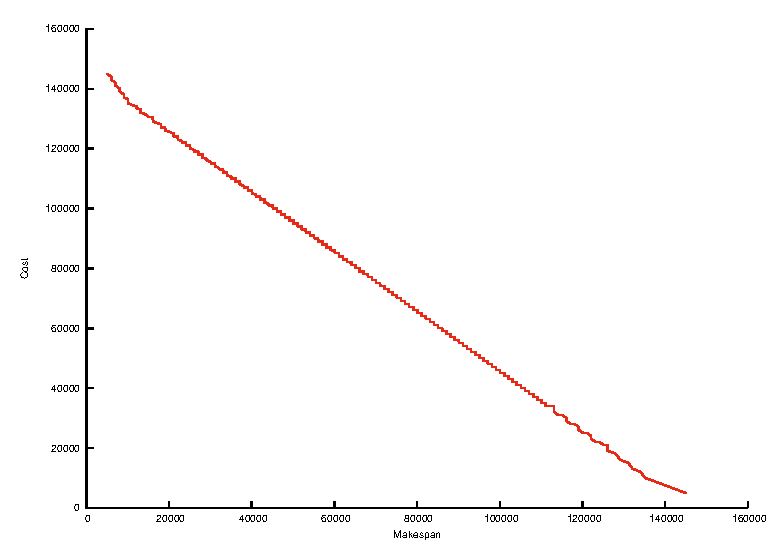
\includegraphics[width=0.30\textwidth]{1}
%       \includegraphics[width=0.30\textwidth]{1+zoom}
%  \caption{\label{instance1} Instance 1: the trend appears to be linear with some convex parts on extremities. However, a zoom shows a totaly unstructured front. {\bf tentative de mettre tout sur 1 seule figure}}
% \end{figure}
% \begin{figure}[h!]
%   \centering
%       \includegraphics[width=0.30\textwidth]{4}
%       \includegraphics[width=0.30\textwidth]{4_zoom}
%  \caption{\label{instance2} Instance 2: a convex trend. The lower part is totally linear while the upper part is made of regular concave patterns.}
% \end{figure}
% \begin{figure}[h!]
%   \centering
%       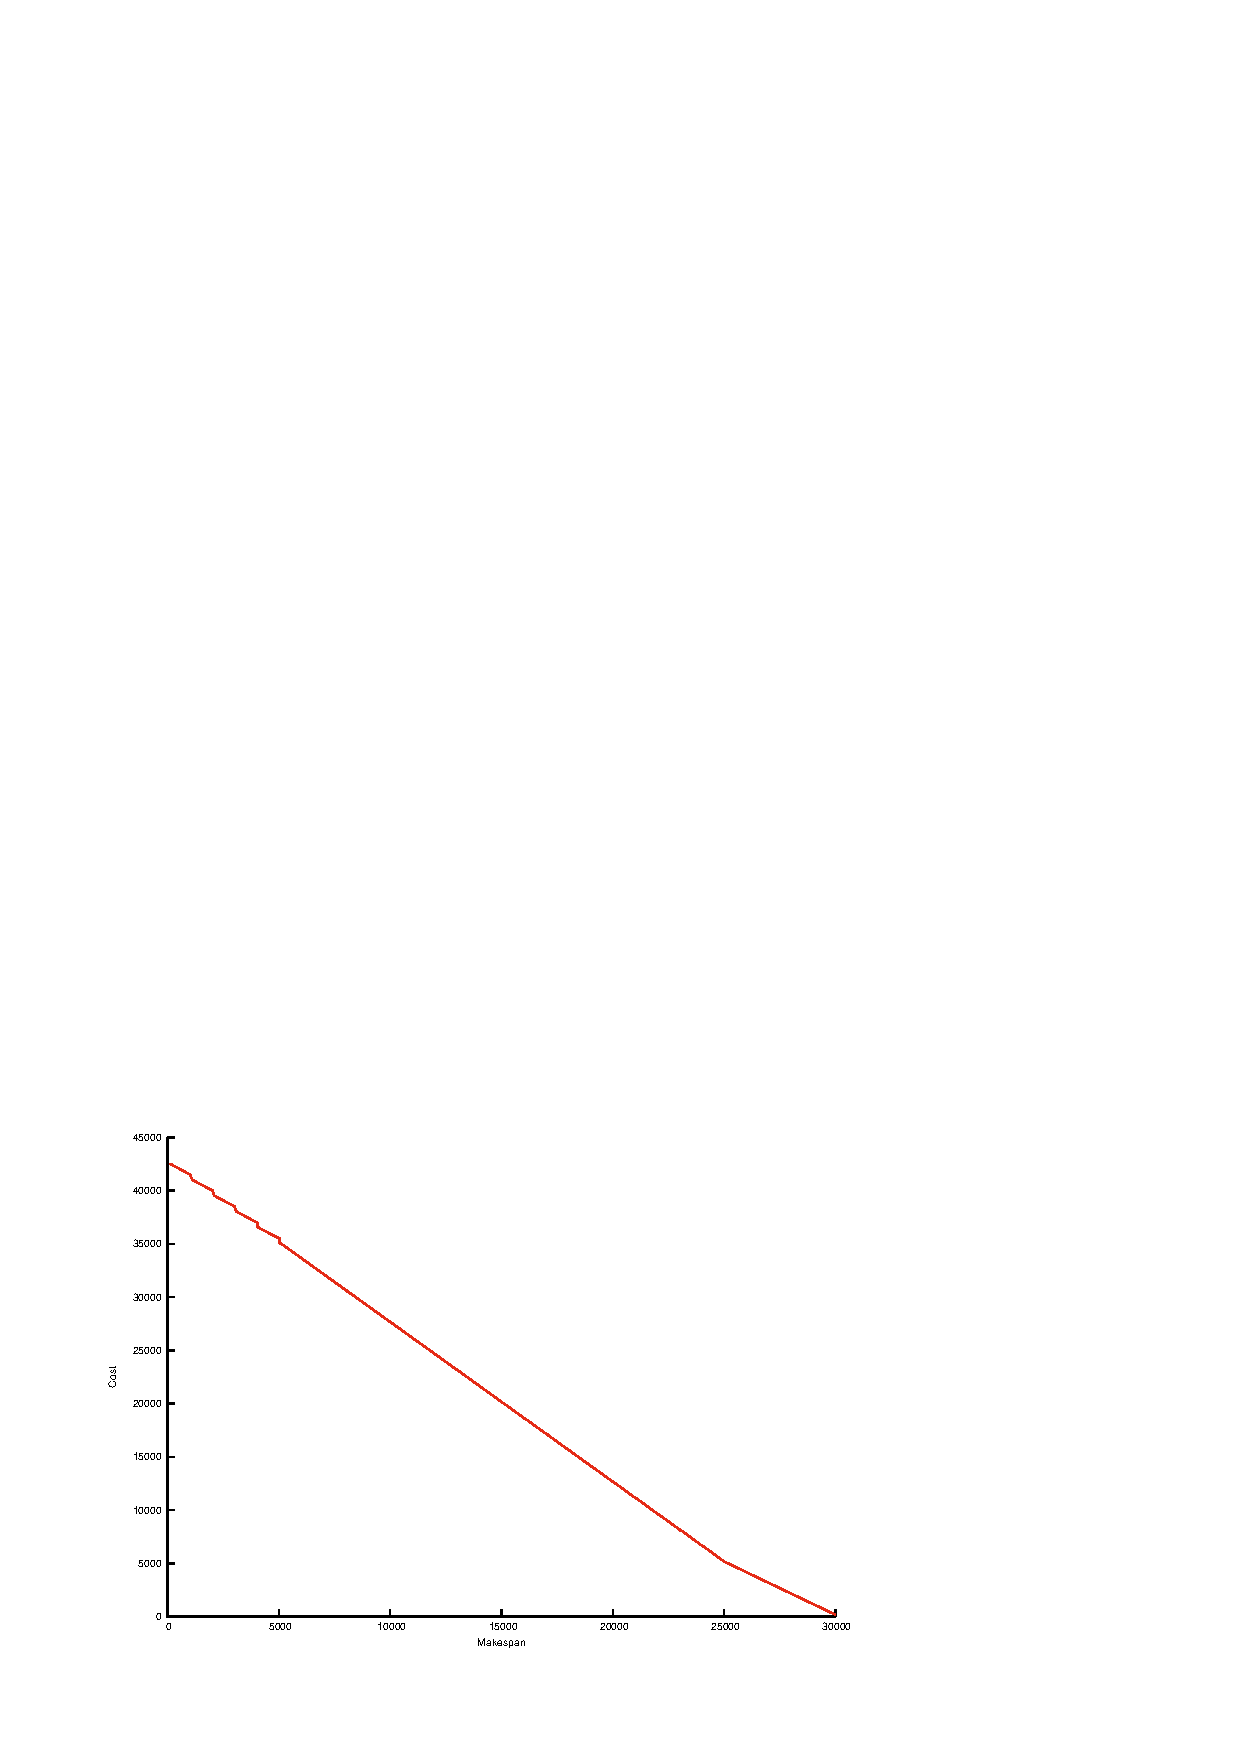
\includegraphics[width=0.30\textwidth]{9}
%       \includegraphics[width=0.30\textwidth]{9_zoom}
%  \caption{\label{instance6} Instance 3: quite linear, a zoom shows a non uniform repartition of points. Clusters of points seems to be regular all over the front.}
% \end{figure}
% \begin{figure}[h!]
%   \centering
%       \includegraphics[width=0.30\textwidth]{6}
%       \includegraphics[width=0.30\textwidth]{6_zoom}
%  \caption{\label{instance3} Instance 4: a concave trend. The lower part is quite regular while the upper part shows a non uniform and non regular distribution of points. We also notice a smaller concave part in the middle of the front that breaks the symmetry of the general trend.}
% \end{figure}
% \begin{figure}[h!]
%   \centering
%       \includegraphics[width=0.30\textwidth]{8}
%       \includegraphics[width=0.30\textwidth]{8_zoom}
%  \caption{\label{instance4} Instance 5: it looks like Instance 3. However, the distribution of points is regular and uniform.}
% \end{figure}
% \begin{figure}[h!]
%   \centering
%       \includegraphics[width=0.30\textwidth]{7}
%  \caption{\label{instance5} Instance 6: only 15 points in spite of the complexity of the instance: the effect of the ratio $\frac p t$.}
% \end{figure}

\begin{figure}[bt]
  \centering
      \includegraphics[width=0.32\textwidth]{1+zoom} \hfill
      \includegraphics[width=0.32\textwidth]{4+zoom} \hfill
      \includegraphics[width=0.32\textwidth]{9+zoom}\\
      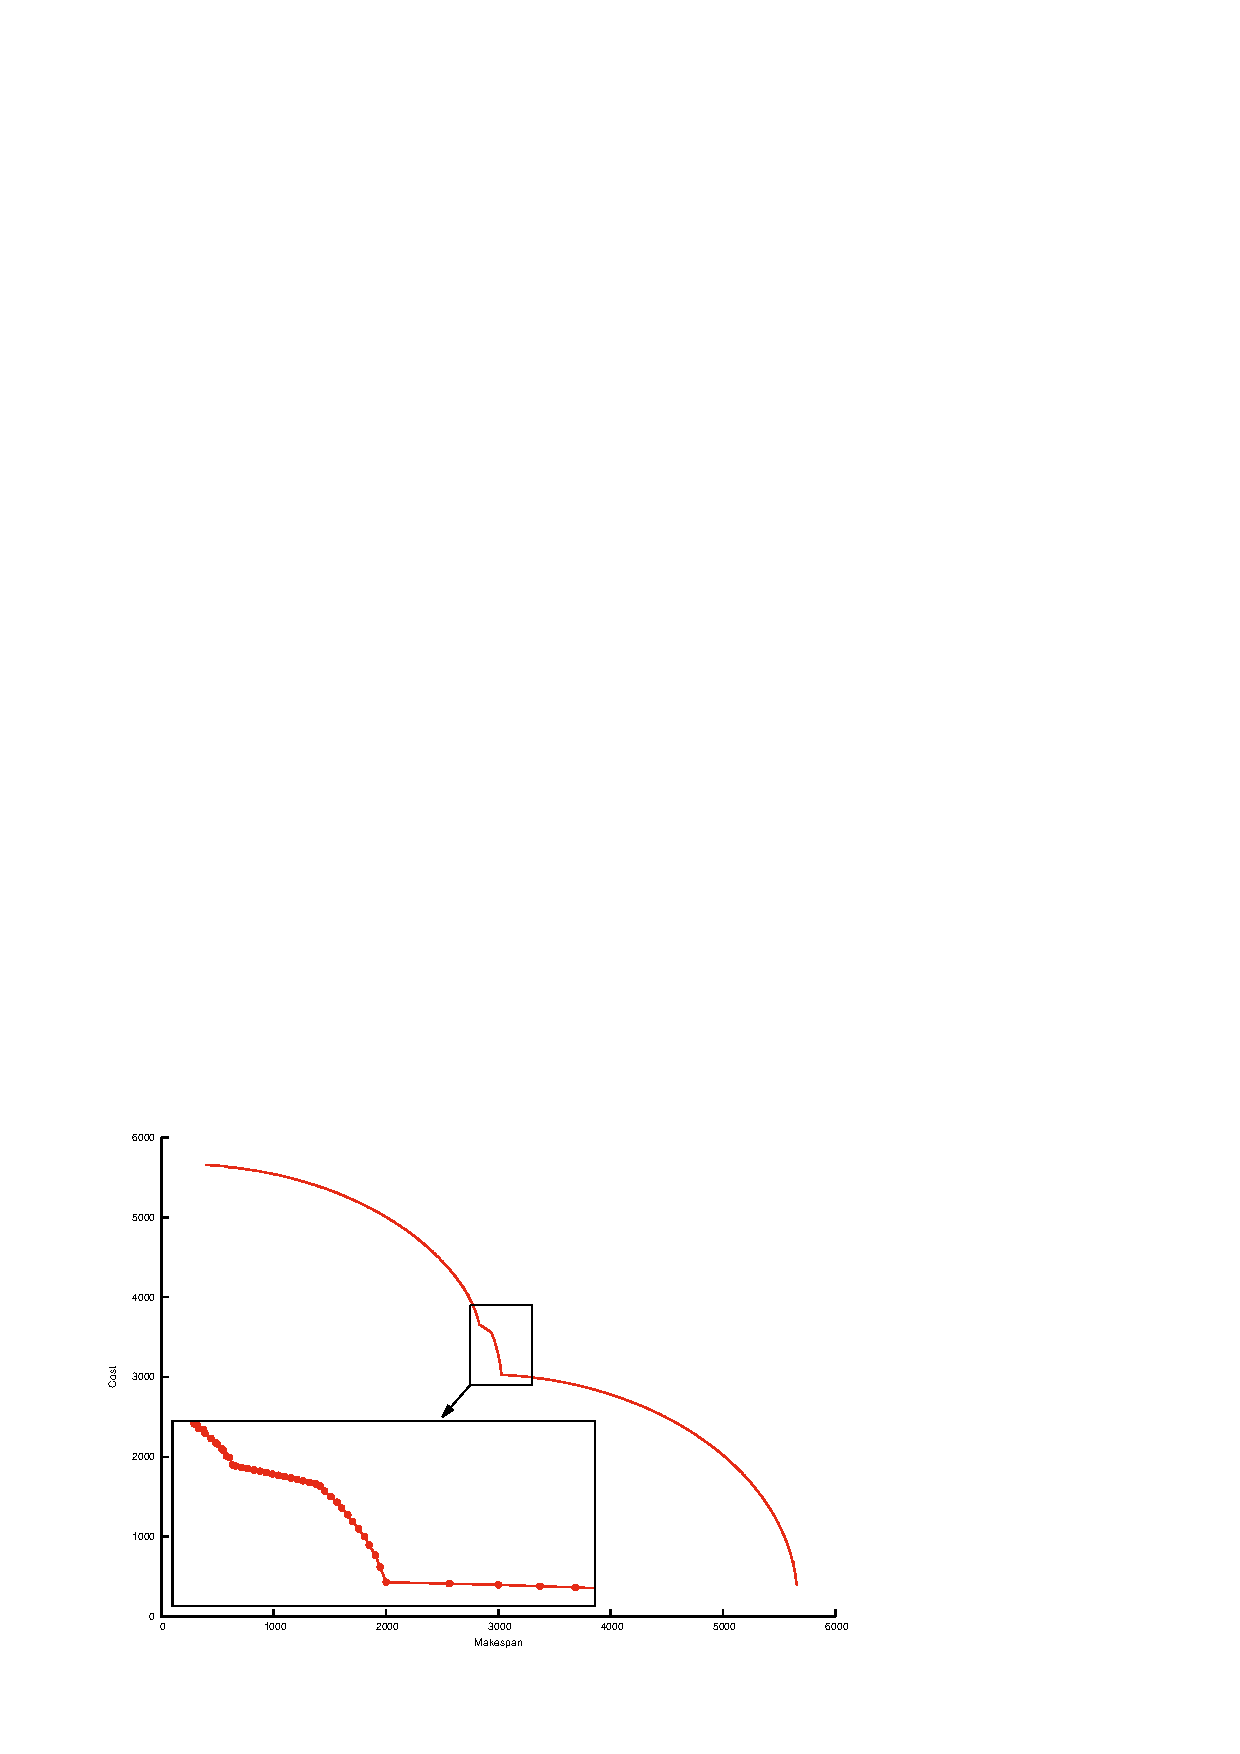
\includegraphics[width=0.32\textwidth]{6+zoom} \hfill
      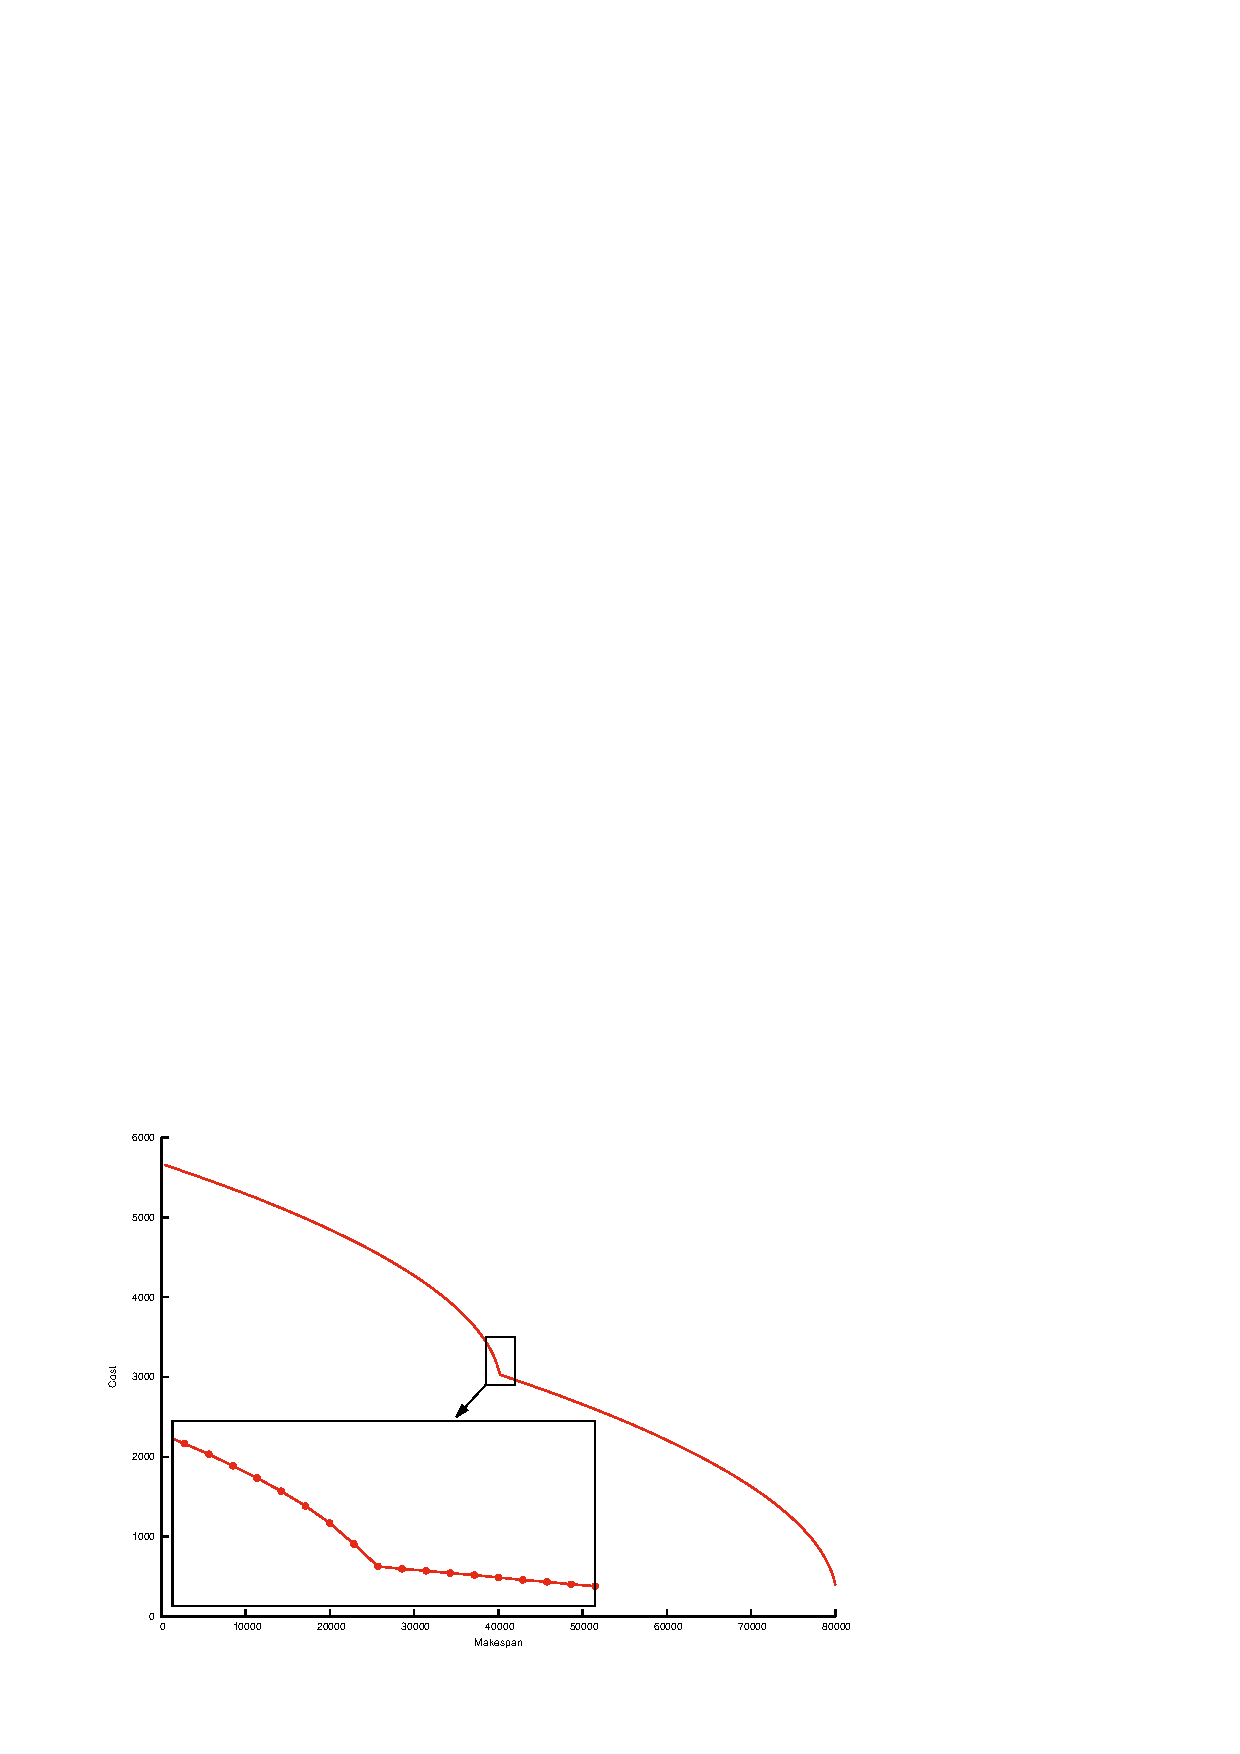
\includegraphics[width=0.32\textwidth]{8+zoom} \hfill
      \includegraphics[width=0.32\textwidth]{7}
\caption{\label{fig:ParetoFronts}True Pareto Fronts for instances 1 to 6 of Table \ref{param}.}
\end{figure}

\begin {table}[tb]
\centering
\caption{\label{param} Sample Large Instances: parameters \& generation statistics.}
\begin{tabular}{|c|c|c|c|c|c|c|c|c|c|c|}
  \hline
  Inst. & Cities & Pass. & Planes & \multicolumn{2}{|c|}{Generating functions} & Pareto\# & $h$ & PPP(k) & Iter.(k)  & Time\\
  \hline
  1 & 20 & 6 & 2 & \multirow{3}{*}{
\begin{tabular}{c}
$\frac{5}{2}i +$ \\
$ \frac{(i ~\text{mod}~ 2)}{10}$
\end{tabular}
} & \multirow{3}{*}{
\begin{tabular}{c}
$\frac{5}{2}i +$ \\
$ \frac{(i ~\text{mod}~ 2)}{10}$
\end{tabular}
} & 409 & 4015 & 1568220 & 3317140 & 16h46\\
  2 & 3 & 21 & 2 &  & & 61 & 861 & 53 & 233 & 2006s\\
  3 & 10 & 10 & 3 & & & 383 & & & &\\ \hline
  4 & 200 & 3 & 2 & $\sqrt i$ & $\sqrt i$ & 538 & 4963 & 270680 & 3906 & 1845s\\
  5 & 200 & 3 & 2 & $\sqrt i$ & $i$ & 399 & 797 & 270680 & 32066 & 1666s\\
  6 & 8 & 26 & 25 & $\sqrt i$ & $i$ & 15 & 190 & 34176 & 60457 & 4240s\\
  \hline
\end{tabular}
\end{table}

% \begin {table}[H]
% \centering
% \caption{\label{genfunc} Generating functions}
% \begin{tabular}{|l|c|c|}
%   \hline
%   Instance & $f$ & $g$ \\
%   \hline
%   Instance 1,2,3 & $f(i) = \frac{5}{2}i + \frac{(i ~\text{mod}~ 2)}{10}$ & $g(i) = \frac{5}{2}i + \frac{(i ~\text{mod}~ 2)}{10}$ \\
%   Instance 4 & $f(i) = log(i)$ & $g(i) = \sqrt i$ \\
%   Instance 5 & $f(i) = log(i)$ & $g(i) = log(i)$ \\
%   Instance 6 & $f(i) = \sqrt i$ & $g(i) = i$ \\
%   
%   \hline
% \end{tabular}
% \end{table}

\section{Multi-objective Experiments}
\label{sec:exp}
\subsection{Divide-and-Evolve}
\label{sec:dae}

Based on the Divide-and-Conquer paradigm, Divide-and-Evolve (\DAE) is a generic hybrid evolutionary originally introduced in~\cite{Schoenauer2006}.   
It splices the problem into a sequence of sub-problems that are hopefully easier to solve by some classical AI planer.
Given a planning problem  ${\cal P}_D(O,G)$ (on domain $D$ with initial state $O$ and target state $T$), the goal is to find an optimal sequence of states $S_0=O, S_1, \ldots, S_n, S_{n+1} \subseteq T$ such that when solving the series of planning problems ${\cal P}_D(S_{k},S_{k+1})$ ($k \in [0,n]$) with some given embedded planer, the sequential concatenation of all sub-plans is an optimal plan for the original problem ($G \subseteq T$). An evolutionary algorithm using specific variation operators is used to evolve the  sequence $(S_i)_{i \in [1,n]}$. The current version (see \cite{Bibai2010} for details) embeds the sub-optimal but very fast planner \YAHSP~\cite{Vidal2004}.

% Our algorithms have been hybridized with an external ’embedded’ planner to solve the sequence of problems ${\cal P}_D(S_{k},S_{k+1})$,  for $k \in [0,n]$. 
% Any existing planner can be used as embedded planner, but since guaranty of optimality at all calls is not mandatory in order for \DAE\ to obtain good quality results~\cite{Bibai2010}, a sub-optimal, but fast planner is used: \YAHSP~\cite{Vidal2004} is a lookahead 
% strategy planning system for sub-optimal planning which uses the  actions in the relaxed plan to compute reachable states in order to speed up the search process.

% \vspace{-1cm}
\subsection{Experimental Conditions}

Previous work \cite{khouadjia:hal-00750560} showed that IBEA$_{H^-}$ performed best among several competitors as the evolutionary engine for \DAEYAHSP. Hence all experiments have been conducted with IBEA$_{H^-}$. DAE$_{\text{YASHP}}$ internal parameters have been tuned thanks to \PARAMILS\ using an {\bf Hypervolume Difference Indicator} metric $H^-$ as detailed in \cite{khouadjia:hal-00820634}. For each instance, 20 independent runs limited to 5400 seconds (1800 for instance 6) have been run. All performance assessments and comparisons have been done using PISA\footnote{http://www.tik.ee.ethz.ch/pisa/}. %\cite{Bleuler2003}.

\subsection{\DAEYAHSP\ on Large Instances}
\vspace{-0.1cm}
The attainment surface on Instance 1 (Figure \ref{attainment1}-left) shows a good fit to the true  Pareto front, even though very few Pareto optima were actually reached (the darker, the larger the probability to reach that region - full white meaning that none of the 20 runs ever reached it). However, the attainment surfaces are uniformly distributed over the front. Surfaces on Instance 2 and 3 are far from the exact front and only 2 points are found for Instance 3 out of 383. On the opposite, even if with smaller budget, most of the actual Pareto optima are found for Instance 6, except on the most concave part. 

We can notice that, even if $n$ is higher for the Instance 6 than for the Instance 2, more planes results in a easier front to reach. This is quite surprising since the search space for \DAEYAHSP\ is growing up with $p$. A reason could be the maximum number of states in a decomposition that has been fixed at 20 and could be too low to obtain easy-to-solve sub-problems, resulting on poor results on the Instance 2 and 3.

% \begin{figure}[h!]
%   \centering
%       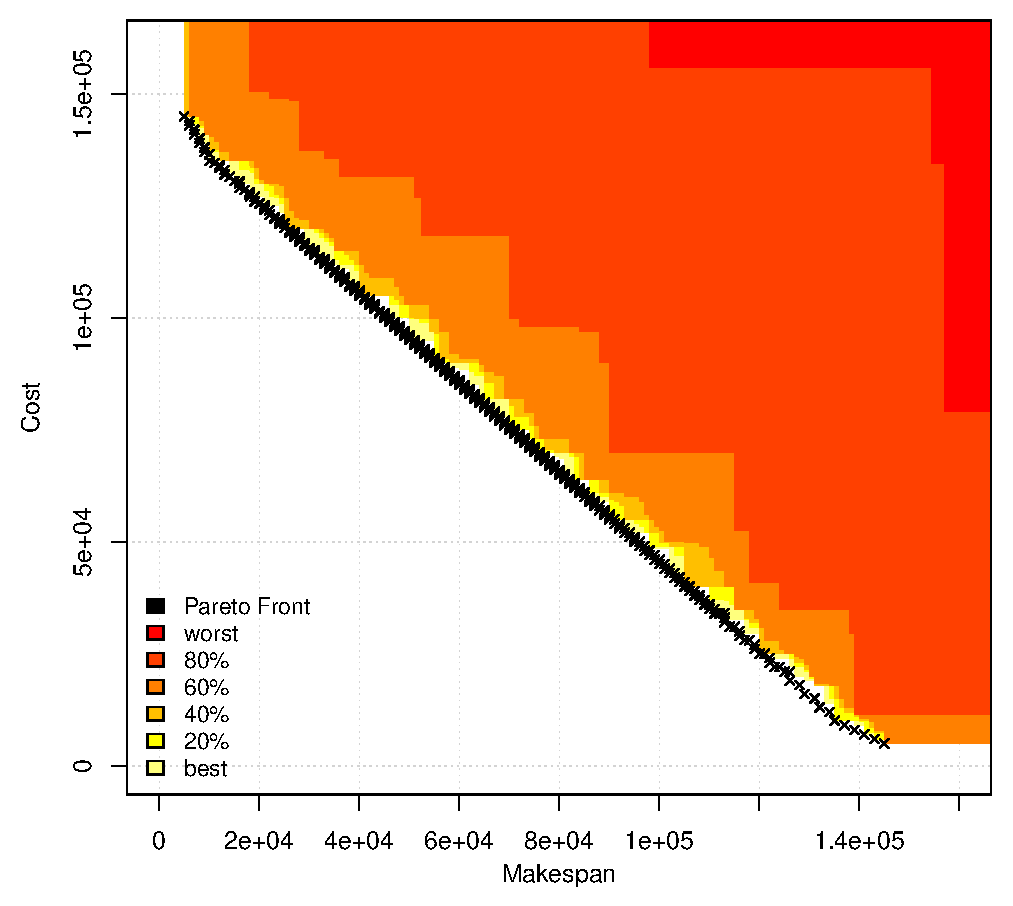
\includegraphics[width=0.30\textwidth]{large_1_att_area}
%       \includegraphics[width=0.35\textwidth]{large_1_hyp}
%  \caption{\label{attainment1} Attainment surface and Hypervolume for Instance 1}
% \end{figure}

\begin{figure}[tb]
  \centering
      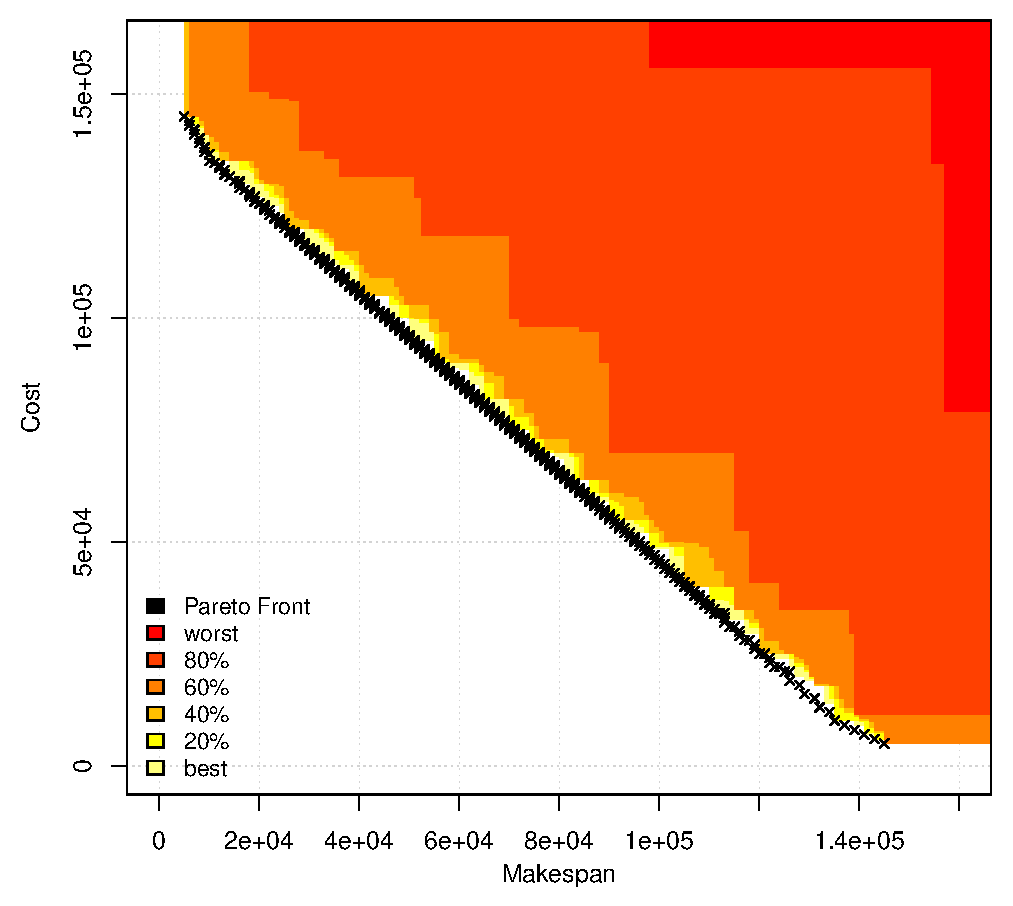
\includegraphics[width=0.24\textwidth]{large_1_att_area}
      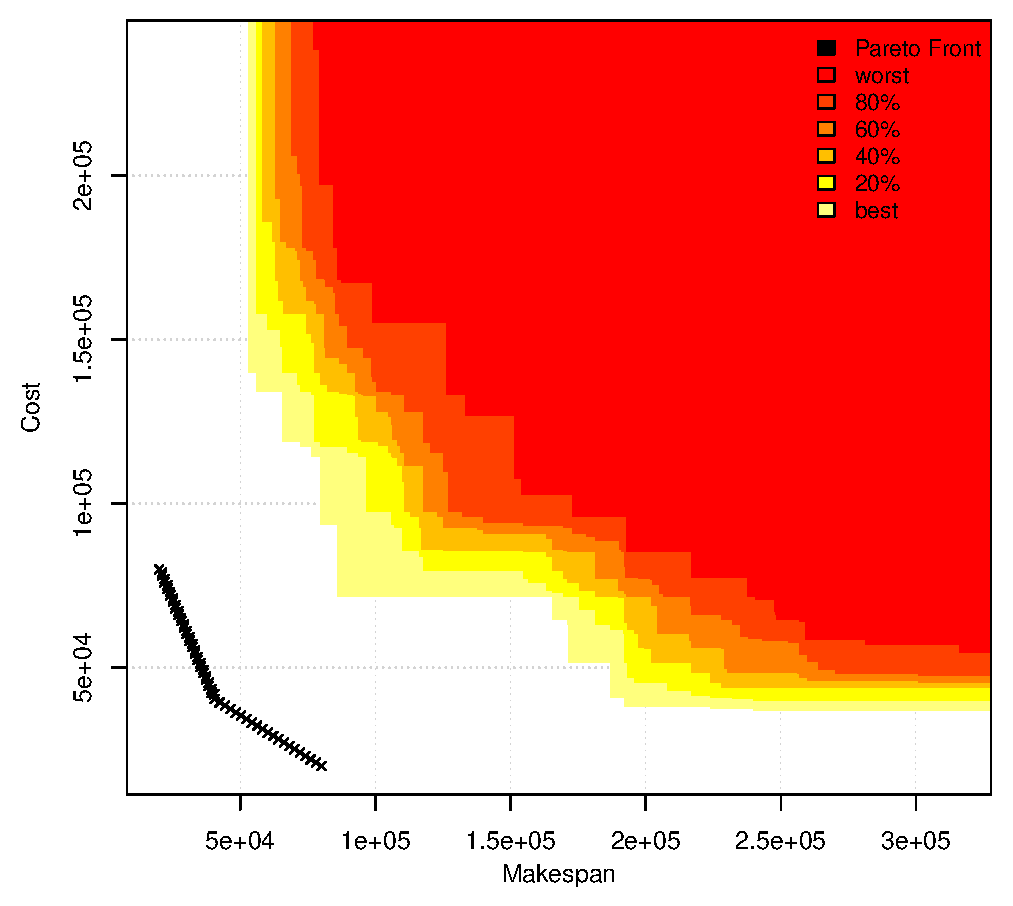
\includegraphics[width=0.24\textwidth]{large_4_att_area}
      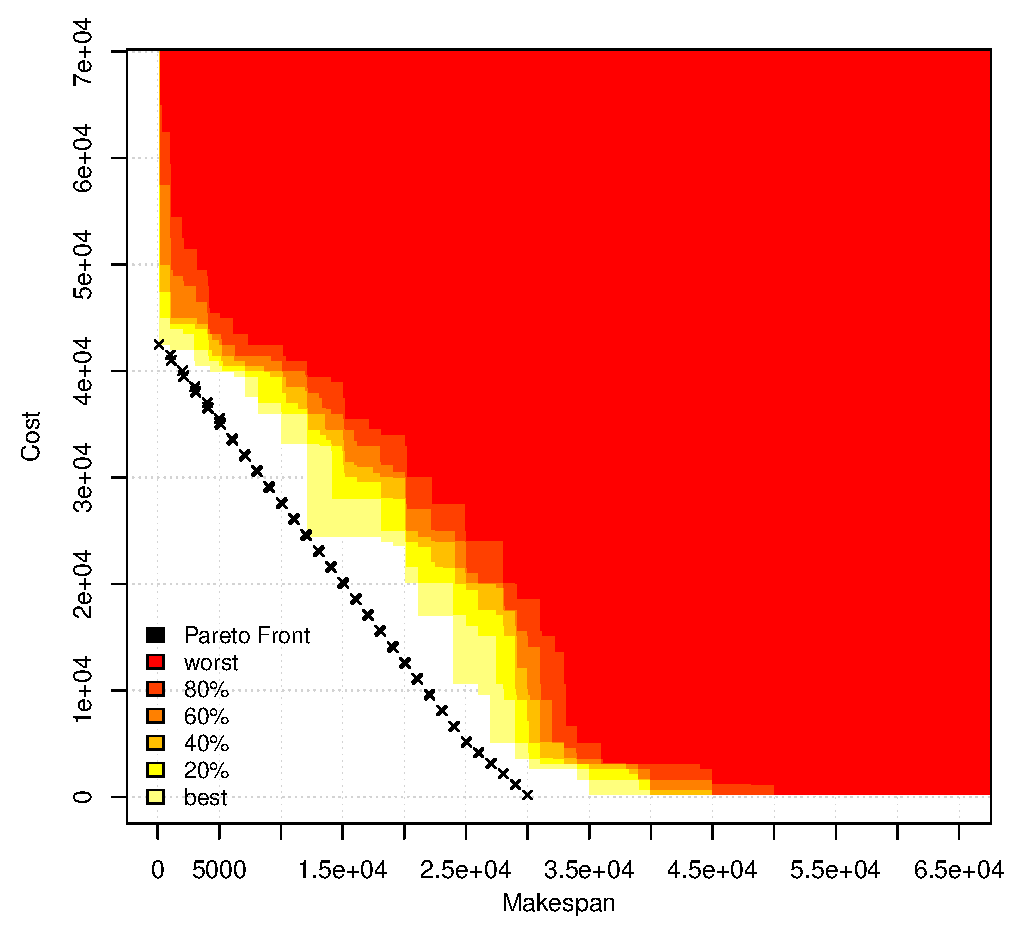
\includegraphics[width=0.24\textwidth]{large_9_att_area}
      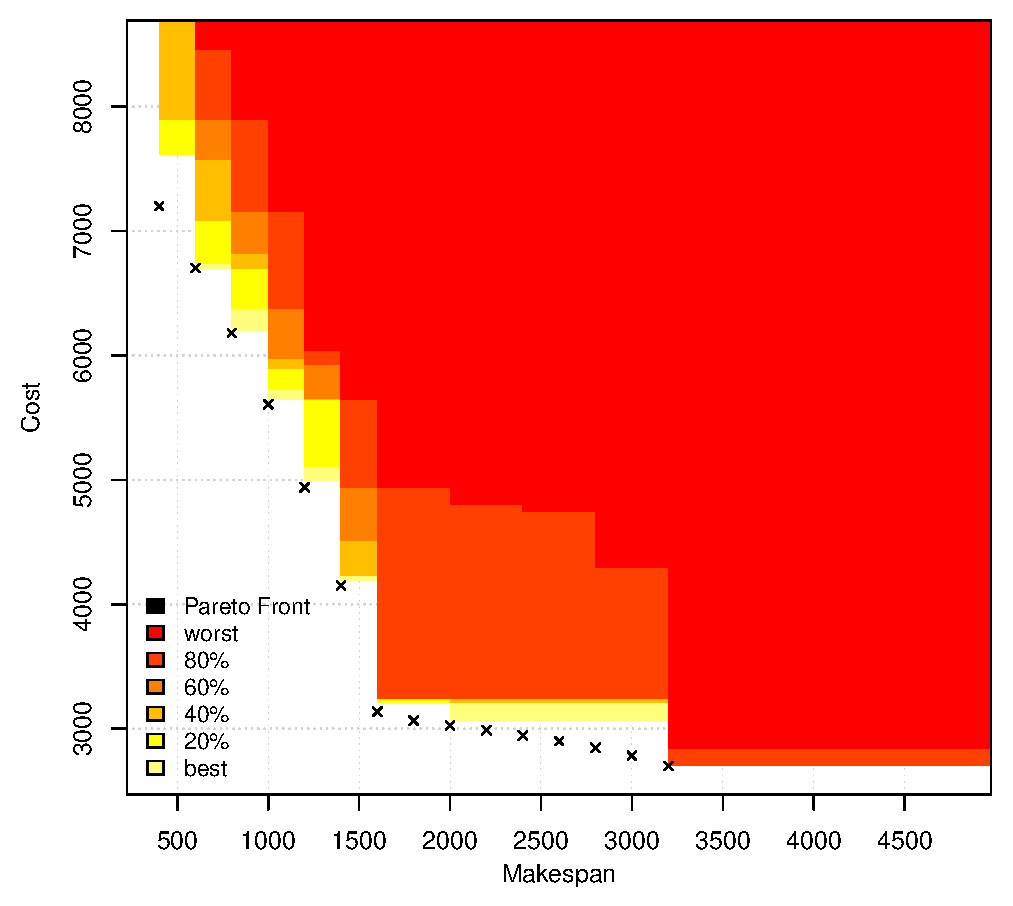
\includegraphics[width=0.24\textwidth]{large_7_att_area}
 \caption{\label{attainment1} Attainment Surfaces and true Pareto fronts for Instances 1, 2, 3 and 6.}
\end{figure}

\subsection{Pareto vs Weighted Sum Aggregation}

Finally, let us have a quick look at some comparative results between the multi-objective version of \DAEYAHSP\ and the single-objective version of \DAEYAHSP\ on a weighted sum of the objectives. 
The chosen instance is a concave instance similar to Instance 4, but with only 30 cities (resulting in a Pareto Front made of 66 points). 
All experimental conditions are the same than in \cite{khouadjia:hal-00820634}. 
One aggregated run amounts to 11 independent runs, the weight parameter $\alpha$ taking values from $0$ to $1$ by step of $0.1$. However, whereas each Pareto run had a budget of 5400s, the same budget was given to each of the $\alpha$-runs (resulting in a total budget 11 times larger for each aggregated run). 

Despite this big advantage, the attainment surfaces (Figure \ref{medium_eaf}) show that in the case of Pareto approach, the exact Pareto Front is already delineated after 900s, even considering only the worst of the 20 runs. On the opposite, even the best of the 20 runs is still far from Pareto Front apart from a few points that lie in the convex parts of the front.
% , as confirmed by the accumulated fronts (merge of the fronts obtained by the 20 runs) on Figure \ref{medium_cum}.
% These trends, though preliminary here, nevertheless confirm the well-known fact that weight sum aggregation has difficulties to reach the concave parts of Pareto fronts.


\begin{figure}[tb]
  \centering
      \includegraphics[width=0.30\textwidth]{medium_att_area_EAFALL_900}
      \includegraphics[width=0.30\textwidth]{medium_att_area_EAFALL}
      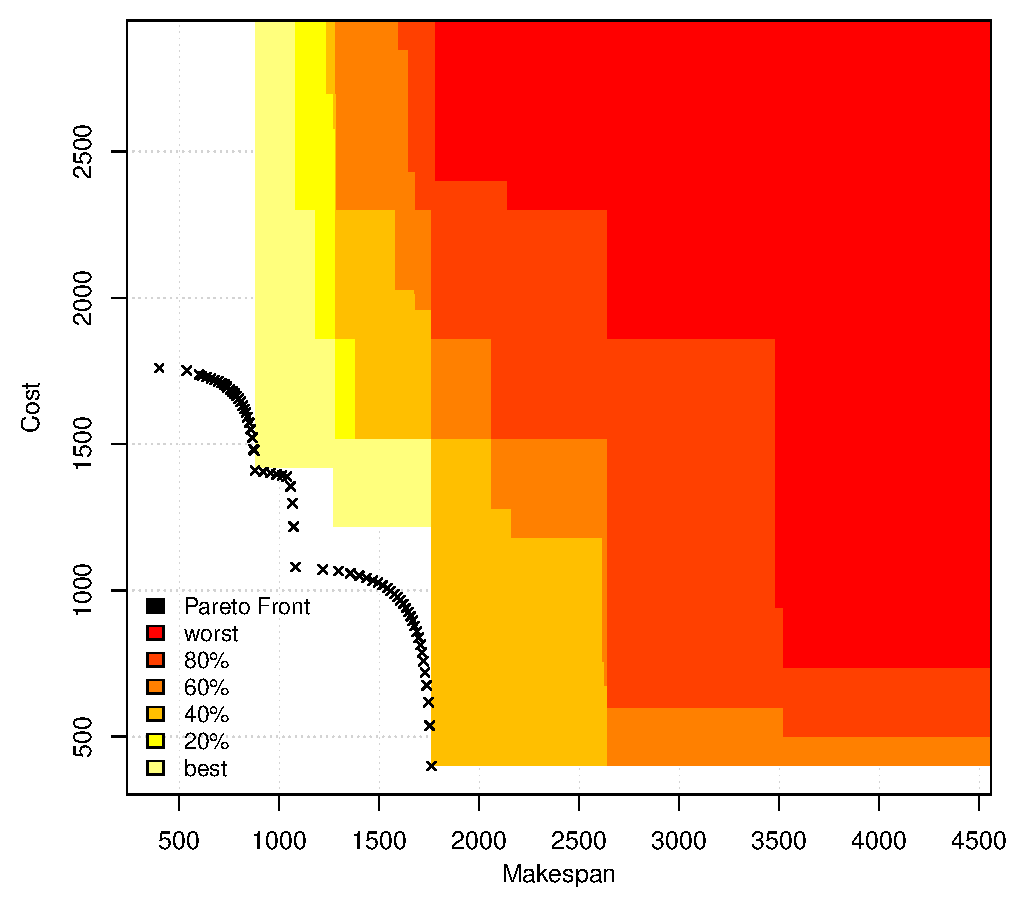
\includegraphics[width=0.30\textwidth]{medium_aggreg_att_area}
 \caption{\label{medium_eaf} Attainment surface for Pareto approach after 900s and 5400s (left, center) and for aggregation after 5400s (right) on (a small version of) Instance 4.}
\end{figure}

% \begin{figure}[tb]
%   \centering
%       \includegraphics[width=0.35\textwidth]{medium_cumulated}
%       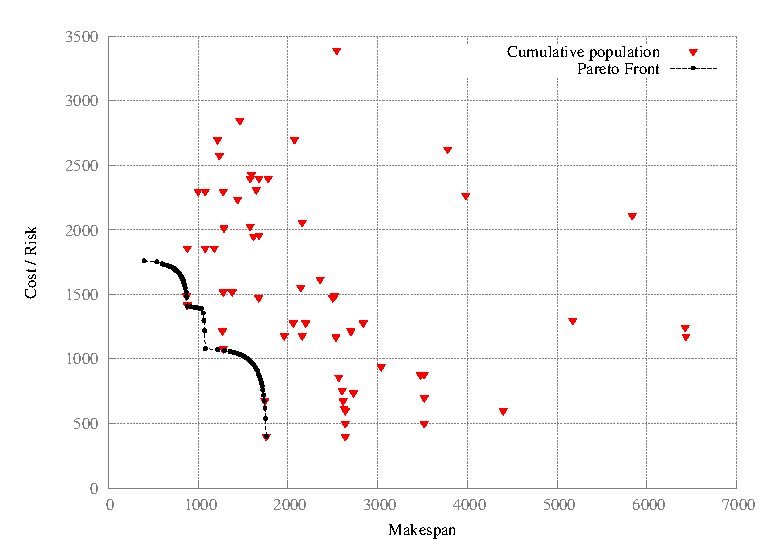
\includegraphics[width=0.35\textwidth]{medium_aggreg_cumulated}
%  \caption{\label{medium_cum} Accumulated Pareto fronts for Pareto (left) and aggregation (right).}
% \end{figure}

% The EAF difference plot indicates attainment surfaces more likely to be reached by an algorithm compare to another. On this concave instance, the parts in favor of the Pareto approach are always closer to the exact front that for the aggregation one. Thus, it is clear that the Pareto approach strongly outperforms the aggregation one and point out the difficulty of aggregation methods to reach concave parts of Pareto Front.

% \begin{figure}[h!]
%   \centering
%       
%       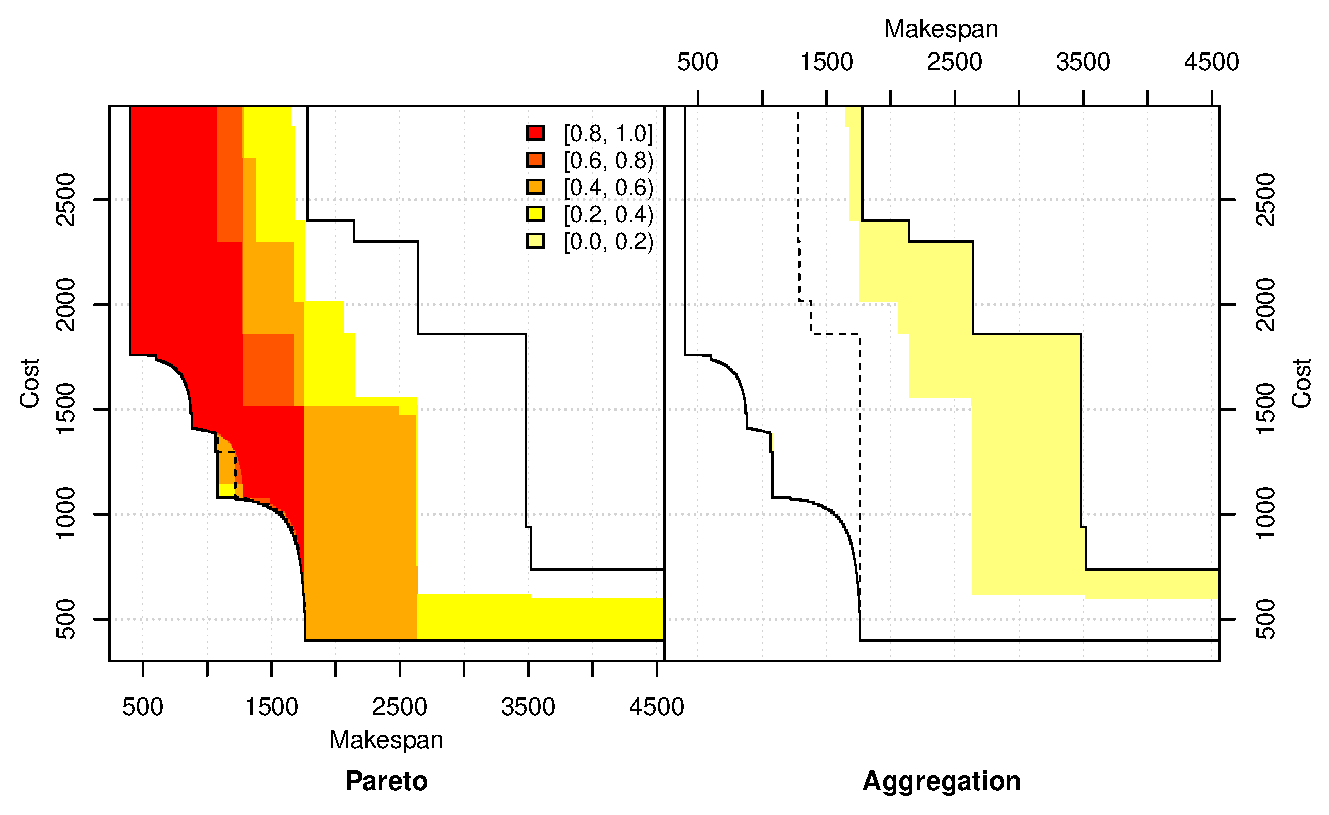
\includegraphics[width=0.6\textwidth]{medium_eaf_diff}
%  \caption{\label{medium_diff} EAF difference between Pareto and Aggregation approches.}
% \end{figure}

\section{Discussion and Perspectives}
\label{sec:conclusion}
The proposed benchmark suite opens the floor to deeper comparative experiments in a combinatorial domain where no ground truth existed for large instances as far as we know.
In particular, beyond the basic weighted sum aggregation used here as a baseline (all $\alpha$-runs are independent), deeper experiments should be made with state-of-the-art decomposition methods in which the different components of the decomposition cooperate (e.g., from the MOEA/D family \cite{Zhang-MOEAD-TEC07}). Thanks to the proposed \MULTIZENO\ benchmark and \ZENOSOLVER\  algorithm (available at \url{https://descarwin.lri.fr}), such experiments can now be made with the knowledge of the ground truth (the Pareto front). In the AI planning domain, this will hopefully lead to sound comparisons between Pareto and non-Pareto planners (see e.g., \cite{LPG-STAIRS2012}).

%
% ---- Bibliography ----
%
\bibliographystyle{splncs03}
\bibliography{ppsnb}
%
\end{document}

%%%%%%%%%%%%%%%%%%%%%%%%%%%%
{\bf Hypothesis}: weights (i.e durations) in the city network satisfy the triangular inequality: $\forall i,j,k \ \ d_{i,j} \leq d_{i,k}+d_{k,j}$, and we suppose also that $\forall i, c_i > 0$ and $d_i > 0$.

\noindent
{\bf Proposition}: Given a path $p_0=(I, i, G), \nexists j$ such that $p=(I, i, j, G)$ with $c(p) > c(p_0)$ and $d(p) < d(p_0)$

\noindent
{\bf Proof}:\\
$d(p_0)=d_i+d_i$\\
$d(p)=d_i+d_{i,j}+d_j$\\
$c(p_0)=c_i$\\
$c(p)=c_i+c_j$\\
Let's suppose that $d(p) < d(p_0)$\\
equivalent to $d_i+d_{i,j}+d_j < d_i+d_i$\\
equivalent to $d_i > d_{i,j}+d_j$\\
but the triangular inequality tells us that $ d_i \leq d_{i,j}+d_j$\\
Which is contradictory.\hfill $\square$

Hence, all $p$ paths (i.e. plans) are dominated by $p_0$ paths.
Hence, there are no flights between central cities in Pareto-optimal plans.
\\
\\
\\
%%%%%%%%%%%%%%%%%%%%%%%%